\documentclass[11pt,a4paper,english]{article}
\usepackage{babel}
\usepackage[utf8]{inputenc}
\usepackage{amsmath}
\usepackage{amsfonts}
\usepackage{amssymb}
\usepackage{graphicx}
\usepackage{natbib}
\usepackage{bbm}
\usepackage{tabularx,booktabs}
\newcommand\numberthis{\stepcounter{equation}{}\tag{Equation \theequation}}
\newcolumntype{B}{>{\centering\arraybackslash}X}

\addtolength{\oddsidemargin}{-.895in}
	\addtolength{\evensidemargin}{-.895in}
	\addtolength{\textwidth}{1.75in}

\addtolength{\topmargin}{-1.25in}
	\addtolength{\textheight}{1.75in}

%\author{Joelle Mbatchou}
\title{Using MCMC based approach for retrospective association mapping with binary traits in structured samples}
%\date{\vspace{-6ex}Oct. $9^{\text{th}}$ 2015}
\date{\vspace{-7ex}}
\begin{document}
\maketitle

The sample constitutes of 45 3-generations families (unless stated otherwise) with 22 individuals in each family ($n=990$). Given the covariates and genotypes, we generate the binary phenotype according to the following logistic mixed model
\begin{align*}
Y_i|\pi_i &\sim \text{Ber}(\pi_i),\\
\text{logit}(\pi_i) &=  \;\beta_0 + \beta_1\, \text{age}_i + \beta_2\, \text{sex}_i + \beta_3\, \text{Z}_i \numberthis\\
&\;\;\; +\lambda \mathbbm{1}_{\{W_{1i}\,>\,0,W_{2i}\,>\,0\}} + U_i,\\
 \mathbf{U} &\sim \; MVN(0, \sigma_a^2\, \Phi),
\end{align*}
where we include the genotype vectors of two causal unobserved common variants $\mathbf{W}_1$ and $\mathbf{W}_2$ (MAF is 0.1 and 0.2 respectively) coded as 0,1 or 2 (i.e. the minor allele count) and $\lambda$ denotes their epistatic effect on the phenotype. Its value corresponds to an increase of about 10\% in the penetrance for individuals that have at least one mutation at both causal loci compared to individuals that don't have any mutation at one (or both) of the two loci. The mean prevalence of the trait is 11\%. We also include three covariates that affect the trait: age, sex and a $N(0,1)$ covariate $\mathbf{Z}$. Families are ascertained based on having at least 5 affected members.

For each setting, we generate 1000 trait replicates and fit the logistic mixed model below using \verb+MCMCglmm+:

\vspace{-5ex}
\begin{align*}
Y_i|\pi_i &\sim \text{Ber}(\pi_i),\\
\text{logit}(\pi_i) &= \textbf{X}_i^\mathrm{T}\boldsymbol{\beta} + U_i\numberthis\\
\mathbf{U} &\sim \; MVN(0, \sigma_a^2\, \Phi),
\end{align*}

\vspace{-1.3ex}
For each trait replicate, 50 markers are generated independently to estimate type 1 error. So there are 50,000 marker replicates used overall to estimate the type 1 error for each method.

The test statistic used for each marker is:
\[
\frac{\mathbf{G}^T\mathbf{H}(\mathbf{Y}-\hat{\pi})}{\hat{\sigma}_G^2 (\mathbf{Y}-\hat{\mathbf{\pi}})^T\mathbf{H}^T\,\Phi \,\mathbf{H}(\mathbf{Y}-\hat{\mathbf{\pi}})}
\]
where $\mathbf{H}$ is a matrix used to center the genotypes (e.g. $(\mathbf{I} - \mathbf{1}\mathbf{1}^T/n)$ for mean centering or $(\mathbf{I} - \Phi^{-1}\mathbf{1}(\mathbf{1}^T\Phi^{-1}\mathbf{1})^{-1}\mathbf{1}^T)$) for centering around the BLUE of allele frequency).

We vary the proportion of variability on the logit scale that's due to the covariates (vs. polygenic effects) from 0 to 100\%. About 40\% of the total trait variability is explained by the covariates and polygenic effects.

\vspace{.25cm}
{\small
\begin{minipage}{.5\textwidth}
\underline{Centering about the mean} (SE = .001)

\begin{verbatim}
Cov/Poly MCMCglmm GMMAT CARAT CERAMIC
 100/0    0.0507 0.0356 0.0509 0.0508
 80/20    0.0493 0.0411 0.0494 0.049
 60/40    0.0503 0.0476 0.0508 0.0506
 40/60    0.0485 0.0477 0.0487 0.0488
 20/80    0.0482 0.0478 0.049  0.0485
 0/100    0.0509 0.0509 0.0504 0.0508
\end{verbatim}
\end{minipage}}
\begin{minipage}{.46\textwidth}
\includegraphics[scale=.45]{mean_center/power_plot.pdf}
\end{minipage}


\vspace{.25cm}
{\small
\begin{minipage}{.5\textwidth}
\underline{Centering about the BLUE} (SE = .001)

\begin{verbatim}
Cov/Poly MCMCglmm GMMAT CARAT CERAMIC
 100/0    0.0519 0.0359 0.0506  0.0505
 80/20    0.0502 0.0418 0.0494  0.0490
 60/40    0.0515 0.0481 0.0504  0.0505
 40/60    0.0524 0.0510 0.0521  0.0521
 20/80    0.0504 0.0496 0.0493  0.0496
 0/100    0.0501 0.0492 0.0497  0.0496
\end{verbatim}
\end{minipage}}
\begin{minipage}{.46\textwidth}
\includegraphics[scale=.45]{BLUE_center/power_plot.pdf}
\end{minipage}


\vspace{.25cm}
{\small
\begin{minipage}{.5\textwidth}
\underline{Using residuals from logistic regression} (SE = .001)

\begin{verbatim}
Cov/Poly MCMCglmm GMMAT CARAT CERAMIC
 100/0    0.0505 0.0362 0.0503 0.0504
 80/20    0.0507 0.0427 0.0507 0.0506
 60/40    0.05   0.0483 0.0504 0.0501
 40/60    0.0492 0.0478 0.0484 0.0482
 20/80    0.0502 0.0505 0.0507 0.0508
 0/100    0.0501 0.0493 0.0508 0.0503
\end{verbatim}
\end{minipage}}
\begin{minipage}{.46\textwidth}
\includegraphics[scale=.45]{get_orthog_res/power_plot.pdf}
\end{minipage}


\end{document}

\noindent\rule{15cm}{0.4pt}

